%!TEX root = ../dissertation.tex

\chapter{Concepts généraux et État de l'art}
\label{chp:etat_art}


\section{Le diagnostic médicale}

\subsection{Présentation générale}
Le diagnostic médical est défini comme étant le processus permettant de déterminer de quelle maladie ou dysfonctionnement souffre un patient à partir des symptômes et des signes cliniques que ce dernier manifeste. Il vient du grec \textit{gnosis} qui signifie "Connaissance".
Dans la littérature, on parle de \textbf{diagnostic} tout simplement, avec le contexte médical étant implicite.
C'est la méthode par laquelle les professionnels de la santé identifient une maladie comme étant la cause la plus probable de symptômes donnés, l'objectif étant la prise en charge la plus adaptée du patient.


\subsection{Les types de diagnostic médical}
Il existe plusieurs méthodes de diagnostic médical. Toutes ces méthodes s'appuient en général sur ces deux composants:
\begin{itemize}
    \item Le recueil des données. Il s'agit de prendre en compte toutes les données nécessaires à l'établissement d'un diagnostic. Il s'agit notamment des antécédents, des signes et symptômes exprimés par le patient, des paramètres, des examens médicaux.
    \item L'analyse des données recueillies.\end{itemize}

Plusieurs méthodes et techniques sont employées dans une procédure de diagnostic médical:

\subsubsection{Le diagnostic différentiel} \footnote{"Differentiel diagnosis", \textit{Merriam-Webster}, Medical Dictionnary} \footnote{"THe patient history: evidence-based approach To Differential Diagnosis", \textit{Siegenthaler, Walter}, 2011, NY-McGraw Hill}

Cette méthode est basée sur la recherche des différentes maladies possibles à la cause des symptômes exprimés par le patient, suivi par une phase d'élimination à partir des différents tests médicaux et autres données additionnelles. L'objectif est de déterminer à la fin la maladie la plus probable. Cette méthode est souvent appliquée avec l'aide de système automatiques d'aide au diagnostic.

En général, des tests de confirmation sont utilisés après l'identification de la maladie la plus probable, comme les tests d'imagerie médicale, pour confirmer le diagnostic.

\subsubsection{La reconnaissance de pattern}

Dans cette méthode, le consultant se base sur son expérience pour reconnaître un pattern de caractéristiques cliniques. Elle est principalement basée sur le fait que certains signes et symptômes peuvent être directement associés à certaines maladies, sans nécessairement mettre en jeu un processus cognitif plus poussé comme dans le diagnostic différentiel.

Cela peut être la principale méthode utilisée dans les cas où les maladies sont "évidentes", ou l'expérience du consultant peut lui permettre de reconnaître rapidement la maladie. Théoriquement, un certain schéma de signes ou de symptômes peut être directement associé à une certaine thérapie, même sans décision définitive concernant la nature de la maladie, mais un tel compromis comporte un risque substantiel de manquer un diagnostic qui a en fait une thérapie différente, de sorte qu'il peut être limité aux cas où aucun diagnostic ne peut être posé.


\subsection{Les étapes d'un diagnostic médical}

Que ce soit par reconnaissance de pattern ou par diagnostic différentiel, le médecin suit toujours 03 étapes pour établir un diagnostic:

\subsubsection{L'anamnèse}
La première chose qu'un médecin fait lorsqu'il reçoit un patient c'est d'interroger ce dernier. On appelle cela \textbf{l'anamnèse}. Après avoir posé des question génériques au patient comme son âge, le médecin pose des question \textbf{dans un ordre précis}, des questions larges aux questions plus précises:

\begin{itemize}
    \item Quelles sont vos habitudes de vie?
    \item Quels sont vos antécédents médicaux?
    \item Depuis combien de temps avez vous mal à la tête?
    \item etc.
\end{itemize}


\subsubsection{L'examen physique}
Après l'anamnèse, le médecin procède à plusieurs examens physiques qui se déroulent en 04 étapes:
\begin{description}
    \item[L'inspection:] Le médecin vous observe
    \item[La palpation:] Le médecin touche et palpe certaines parties du corps
    \item[La percussion:] Le médecin recherche des bruits anormaux, par exemple en tapant l'arrière du dos
    \item[L'auscultation:] Le médecin écoute certains organes internes (coeur, poumons, etc) à l'aide d'un stéthoscope.
\end{description}

\subsubsection{Les examens complémentaires}
Si c'est nécessaire, le médecin peut demander des examens complémentaires. Un médecin spécialisé pourra par exemple vous faire, ou prescrire une échographie, ou alors un scanner, une radio, une IRM, une biopsie ou un bilan sanguin...

Ces examens  ont pour but de répondre à une \textbf{hypothèse diagnostique}. Chaque examen peut servir à confirmer ou infirmer une question que se pose le médecin, et peut même dans certains cas donner plus d'informations au médecin pour qu'il considère des possibilités auxquelles il n'avait pas pensées en amont.


\subsection{Les challenges}
La médecine fait face à de nombreuses difficultés. Un diagnostic parfois difficile à poser car il faut souvent prendre du temps avant de trouver le diagnostic sur un ensemble de symptômes. Cela est tout à fais concevable car le nombre de symptômes est bien inférieur au nombre de maladies existantes: il existe entre 200 et 300 symptômes, pour plus de 10 000 maladies. Il peut aussi arriver que certains patients n'arrivent tout simplement pas à exprimer leurs symptômes pour de multiples raisons (expression orale, ressenti faussé, peur d'être jugé, ...), ou alors ils omettent tout simplement certains symptômes car jugent qu'ils ne sont pas important. 

Les médecins ont donc une \textbf{obligation de moyens} mais pas de \textbf{résultat}. Un diagnostic n'est donc pas certain et même les examens ne permettent pas d'avoir toutes les informations sur le corps humain. Parfois, il n'est pas possible de poser un diagnostic en dépit des examens réalisés car ces derniers peuvent ne pas répondre aux questions que se pose un médecin. Les symptômes persistent sans que l'on réussisse à identifier la cause. On dit alors que le patient est une \textit{errance diagnostique}.

Toutes ces raisons contribuent au fait que la pose de diagnostic médical est un exercice complexe à réaliser, et demande de la part du médecin des connaissances poussées, une bonne capacité de raisonnement et une très bonne intuition.

\newpage

\section{Les systèmes tutoriels intelligents}

\subsection{Historique et définition}

Après l'avènement des ordinateurs, les progrès technologiques qui ont suivi, ont considérablement augmenté la puissance de calcul de ces derniers. Le gain en performance des ordinateurs a engendré la naissances de nouveaux domaines de recherche parmi lesquels celui qui aujourd'hui suscite le plus d'engouement, à des impacts importants et est l'un des plus prometteurs : l'intelligence artificielle. Dès le début des années 1960, les ordinateurs ont été utilisés à des fins éducatives variées. De même, la formation assistée par ordinateur a rapidement gagné le domaine de l'éducation et le marché de la formation. Dès le début des années 1970, des objectifs ambitieux dans la recherche sur la formation assistée par ordinateur on conduit au développement des premiers systèmes tutoriels intelligents qui ont été obtenus en appliquant les techniques d 'intelligence artificielle pour implémenter un modèle pédagogique basé sur un tuteur humain dans une
formation assistée par ordinateur. Le système tutoriel intelligent remplirait à ce moment la fonction d'engager l'apprenant dans une activité de raisonnement soutenu en interagissant avec lui sur la base d 'une compréhension profonde de son comportement. Le développement des STIs s'est poursuivi depuis jusqu'aux versions de systèmes complexes offrant des formations adaptatives et de qualité que nous retrouvons aujourd'hui.


Un système tutoriel intelligent (STI) peut être définit comme un environnement d'apprentissage informatisé qui intègre des modèles computationnels empruntés aux sciences cognitives , à la linguistique computationnelle, aux sciences de l'éducation , à l'intelligence artificielle, aux mathématiques ainsi qu'à d'autres domaines. Un STI est capable de traquer le comportement de l'apprenant à l'aide d'un processus appelé modélisation de l'apprenant. Le modèle de l'apprenant peut comprendre ses connaissances sur le sujet d'apprentissage, ses compétences, sa stratégie d'apprentissage, son degré de motivation, ses émotions
et d'autres attributs que l'on peut évaluer. Le STI utilise les informations de ce modèle pour interagir avec l'apprenant de manière adaptative. Les STIs ont fait leurs preuves avec le temps et se sont montrés très efficaces notamment dans les domaines des mathématiques, d es sciences et des technologies. Ils représentent un support d'apprentissage ayant un impact nettement plus
important que l'environnement des salles de classes et peuvent captiver l'attention et l'intérêt de l'apprenant pendant des heures.


\subsection{Les composantes d'un STI}


L'architecture de base d'un système tutoriel intelligent est constituée de quatre composantes : le module expert, le module tuteur, le module apprenant et l'interface utilisateur. La figure \autoref{fig:1} inspirée de \cite{nkambou2010advances} présente l'architecture générale d'un système tutoriel intelligent (STI).

\begin{figure}
    \centering
    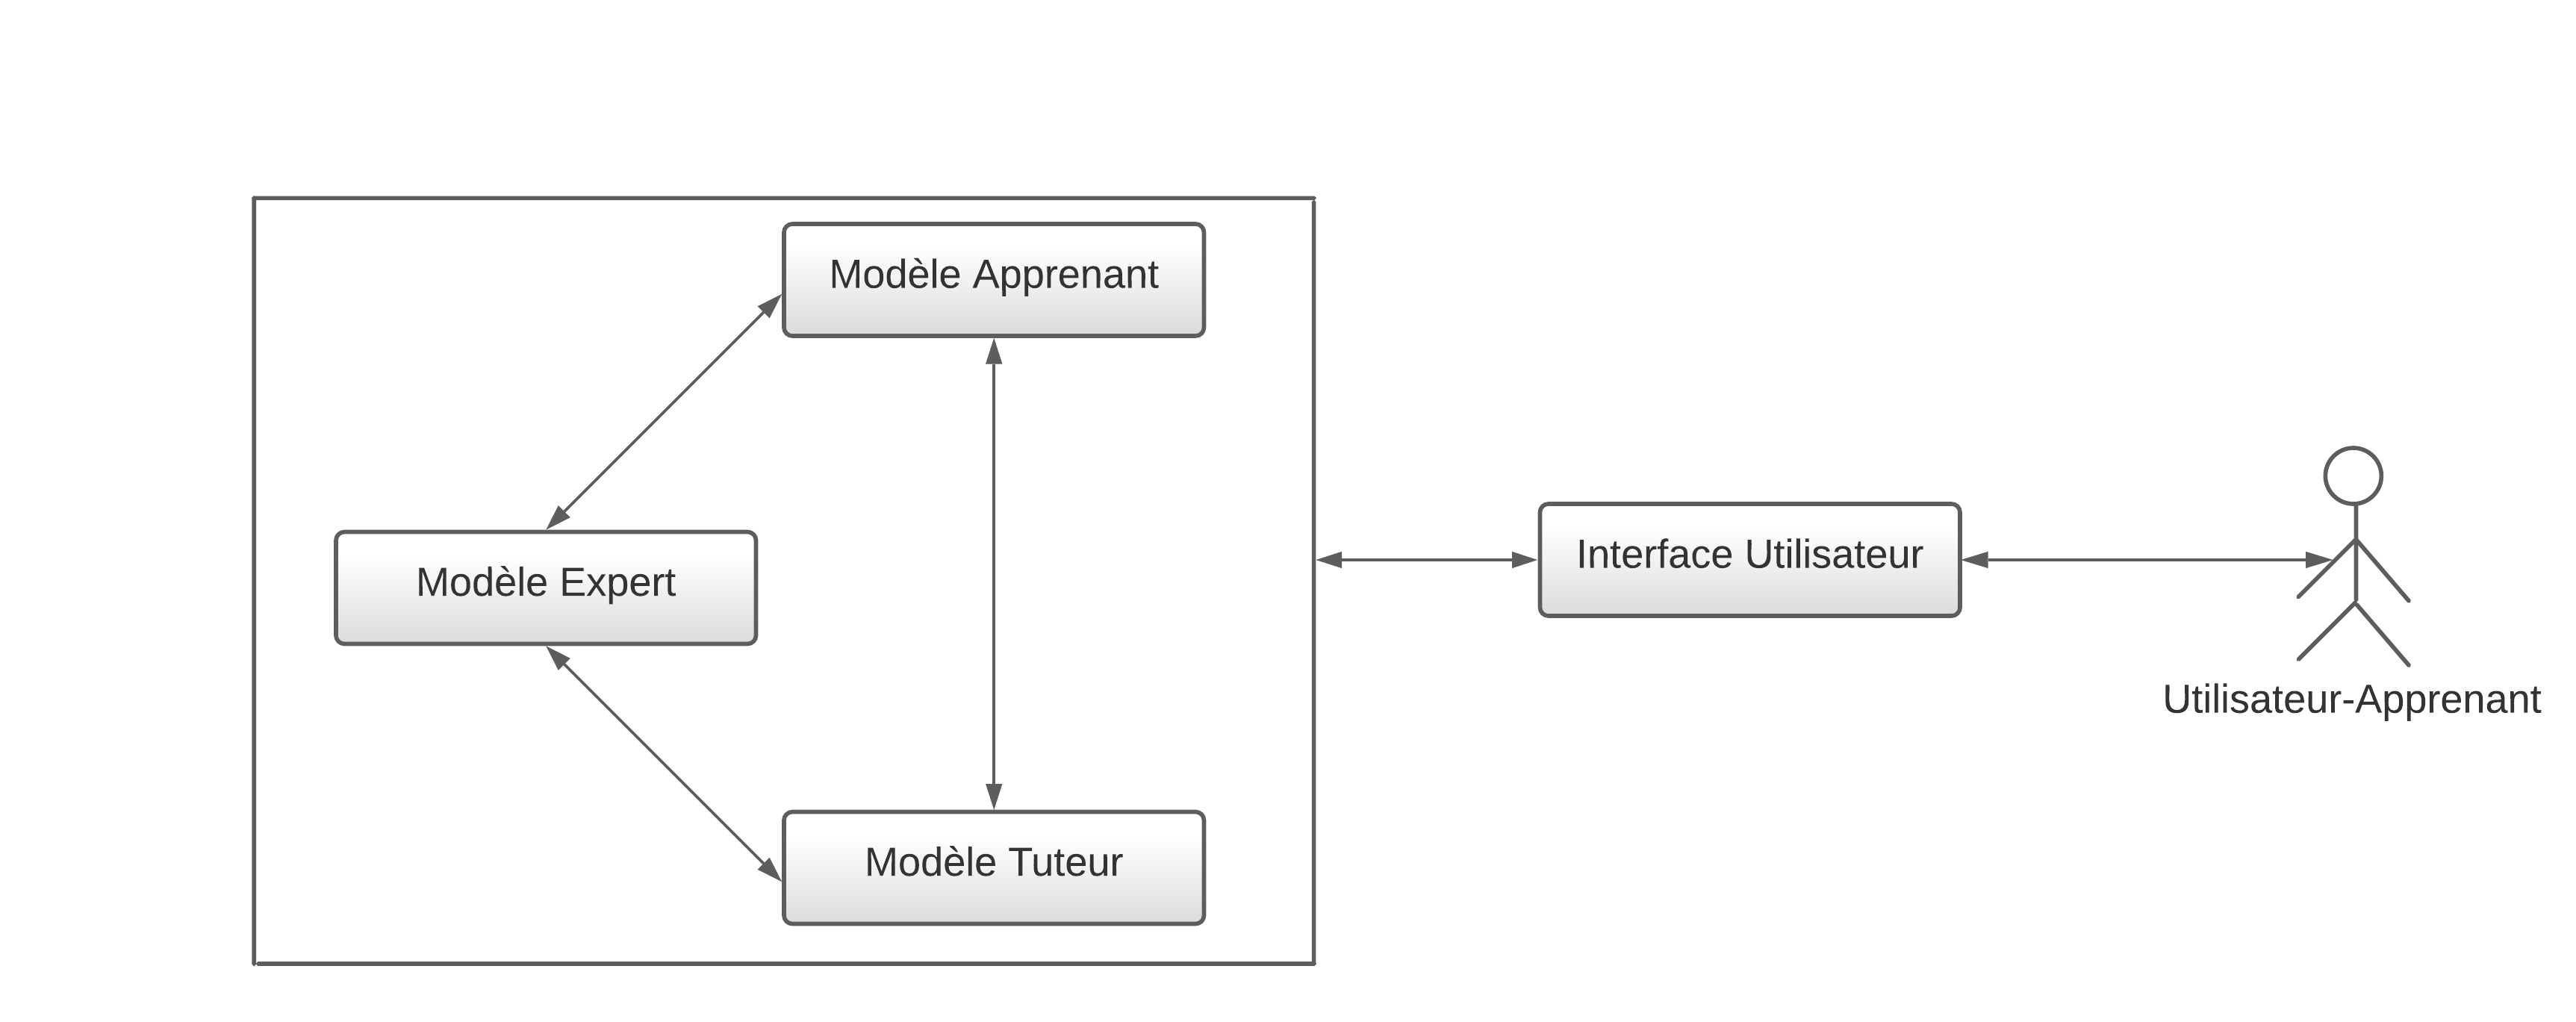
\includegraphics[width=0.9\textwidth]{figures/archi_STI_gen.png}
    \captionsetup{justification=centering}
    \caption{Architecture générale d'un STI}
 \label{fig:1}
\end{figure}


\newpage

\subsubsection{Le module Expert ou module du Domaine}
C'est dans cette composante que sont encodées les connaissances et les mécanismes de résolution de problème du domaine sur lequel porte l'apprentissage. Le module expert d'un STI est assimilable à un expert humain du domaine et doit être capable d'appliquer un raisonnement sur les connaissances encodées, et il doit pouvoir expliquer comment il résout un problème.

L'expert est la source des connaissances à transmettre à l'apprenant. Il fournit par ailleurs au système une norme pour évaluer la performance de l'apprenant détecter ses erreurs ou ses idées fausses.

De part son importance dans le système, son implémentation constitue le plus souvent 50\% des efforts de développement et nécessite de suivre de manière systématique une méthodologie d'ingénierie des connaissances pour garantir la fiabilité et la robustesse du système.

Il existe plusieurs formalismes de représentation des connaissances dans le module expert:
\begin{itemize}
    \item Système de production de règles
    \item Réseaux sémantiques
    \item Représentation procédurale
    \item Représentation basée sur les objets structurés (les \textit{frames}) \footnote{Paquette, 1999}
\end{itemize}

Selon ces différents formalismes, il existe trois approches de modélisation de l'expert du domaine:

\begin{description}
    \item[L'approche "Boite Noire":] Appliquer une quelconque méthode de raisonnement sur le domaine. L'expert fournit les mécanismes de résolution des problèmes et les normes pour évaluer 1 apprenant, mais ne fournit aucune explication sur les démarches suivies pour la résolution des problèmes.
    \item[Système expert:] . L'expert peut au besoin expliquer les démarches de résolution de problèmes. Cette approche offre une représentation articulée des connaissances à la base de l'expertise. 
    \item[Modèle cognitif:] L'expert simule la manière dont l'humain utilise ses connaissances pour résoudre les problèmes.
\end{description}

D'après le diagramme comparatif de la \autoref{fig:diag} \footnote{Nkambou et al., 2010}, l'approche de modélisation du module expert qui démontre la plus grande efficacité pédagogique est le modèle cognitif. Ce modèle nécessite un grand effort d'intégration et constitue le modèle qui se rapproche le plus de l'intelligence humaine.

\begin{figure}
    \centering
    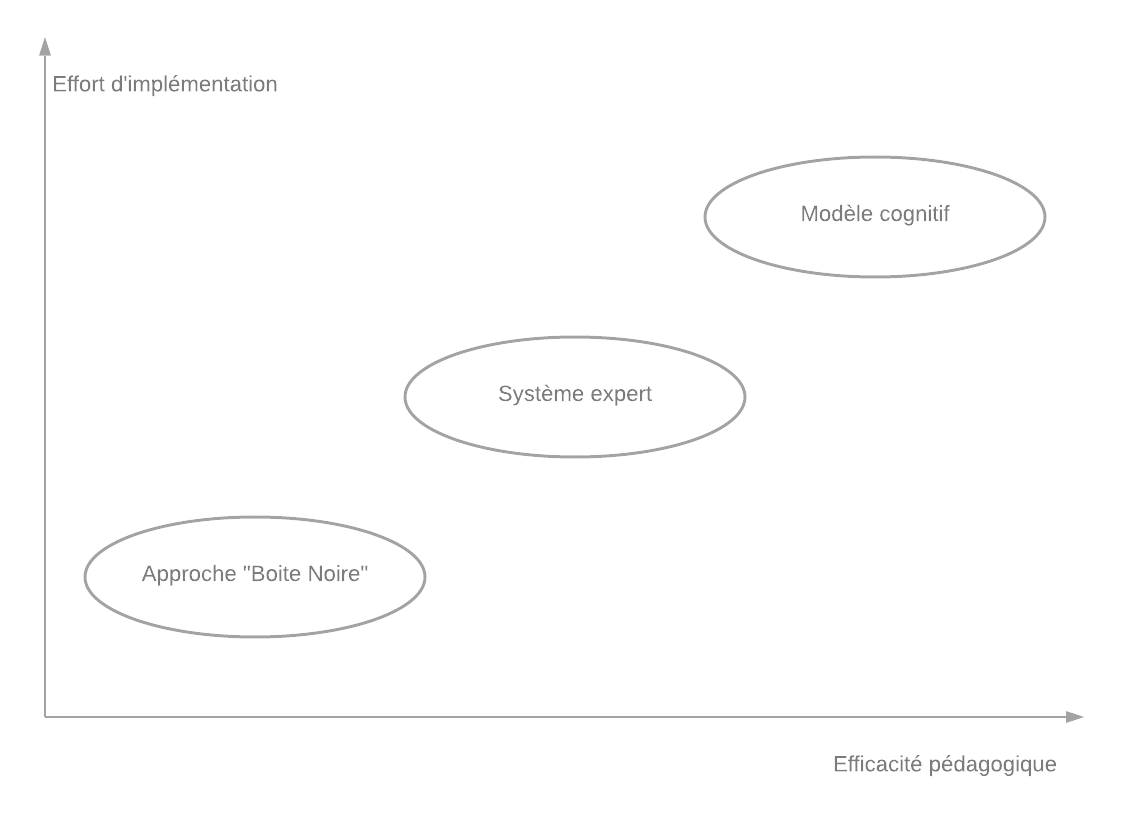
\includegraphics[width=0.9\textwidth]{figures/mod_expert.png}
    \captionsetup{justification=centering}
    \caption{Diagramme comparatif de méthodes de modélisation de l'expert}
 \label{fig:diag}
\end{figure}

\subsubsection{Le module Tuteur}
Le module tuteur est la composante du STI qui implémente les stratégies pédagogiques propres au domaine cible de l'apprentissage . Il interagit avec le module expert et le module apprenant pour choisir et planifier les activités présentées à l'apprenant tout en lui fournissant, le cas échéant, des explications adaptées. Le tuteur décide de quand et comment intervenir selon la stratégie la plus appropriée et en fonction du résultat du diagnostic de l'apprenant (état cognitif, état
émotionnel, niveau d'expertise, connaissances, compétences, forces et faiblesses, etc ...). Il a le choix entre plusieurs stratégies possibles :

\begin{itemize}
    \item Entraînement (Coaching). Le tuteur offre des conseils à l'apprenant et le guide lorsqu'il s'éloigne de la solution.
    \item Apprentissage socratique. Le tuteur propose des exercices mettant en pratique les éléments du domaine pour amener l'apprenant à identifier les règles
de niveau supérieur et les concepts. L'approche vise à faire révéler à l'apprenant ce qu'il possédait déjà sans en être conscient. Ce dernier examine les données immédiates de sa conscience de façon à répondre à des questions
qui la sollicitent et cherche à agir adéquatement à partir de cette conscience
éveillée .
    \item Apprentissage exploratoire. Le tuteur laisse l'apprenant explorer librement
le problème et n'intervient qu'à la demande de ce dernier.
    \item Apprentissage par perturbation.
    \item Apprentissage par auto-explication.
    \item Apprentissage par la pratique. Le tuteur fait quelques démonstrations de
résolution de problème étape par étape, avant de demander à l'apprenant d'effectuer la procédure par lui-même.
    \item Apprentissage par problème. Le tuteur choisi des problèmes qui répondent aux lacunes de l'apprenant.
    \item Etc.
\end{itemize}

Le tuteur s'appuie à chaque fois sur des approche éducatives appropriées pour prendre sa décision. Il supervise l'apprentissage pendant toute la durée de l'activité. Chaque fois que l'apprenant effectue une action ou fournit la réponse à un problème, le tuteur consulte l'expert pour évaluer sa réponse, lui fournit le
feedback approprié selon le contexte et met à jour son modèle (modèle de l'apprenant). Le rôle important que joue le feedback du tuteur dans le processus d'apprentissage a été prouvé et un cadre formel d'élaboration des bonnes stratégies de feedback \cite{narciss2008feedback} a été établi pour maximiser le gain d'apprentissage chez l'apprenant .


\subsubsection{Le module Apprenant}
\textbf{1. Les approches de modélisation de l'apprenant} \\\
Parmi les techniques de modélisation connues. nous pouvons citer :
\begin{itemize}
\item \textbf{Modèle de Recouvrement} \\\
La première approche consiste à construire le modèle de l'apprenant de façon
comparative. Les performances de celui-ci sont comparées à un modèle idéal qui
représente les connaissances d'un expert de la matière enseignée. Carr et Goldstein (1977) appellent cette technique. la méthode de recouvrement des connaissances de l'étudiant « overlay mode1 ». Le modèle de l'apprenant est alors considéré comme un sous ensemble du modèle idéal.
Les connaissances de l'apprenant sont alors considérés comme formant un sous-ensemble des connaissances de l'expert. Le modèle de l'apprenant est alors mis à jour en le comparant au modèle de l'expert. Chaque fois que le modèle de l'apprenant diffère du modèle de celui de l'expert du domaine, le système identifie une erreur ou une idée fausse de l'apprenant.
 La figure 3.1 présente les deux variantes du modèle superposition ( Overlay) : 
 \begin{itemize}
\item une variante dans laquelle les connaissances de l'apprenant sont entièrement incluses dans celles de l'expert (a),
\item une variante dans laquelle sont stockées les informations sur les conceptions erronées de l'apprenant (b).
\end{itemize}
 La deuxième variante permet une meilleure planification des interventions du système dans le processus d'apprentissage. 
 
\begin{figure}
    \centering
    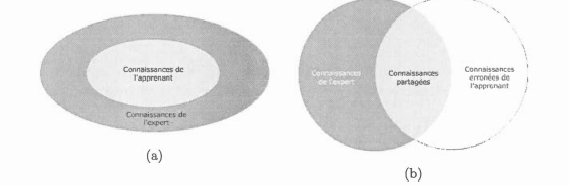
\includegraphics[width=0.9\textwidth]{figures/mdele.png}
    \captionsetup{justification=centering}
    \caption{Les variantes du modèle}
\end{figure}

Il existe plusieurs approches permettant de d'implémenter les superpositions :
 
\begin{itemize}
\item Réseau sémantique. les nœuds et liens sont ajoutés au fur et à mesure que les concepts sont appris par l' étudiant ; 
\item Banque de connaissance de l’expert :  Annoter des déviations que l'on découvre au fur et à mesure de l'interaction avec l'apprenant. 
Ensemble des compétences acquises par l 'étudiant.  Les compétences sont construites sur les éléments de connaissance du domaine. Elles indiquent clairement l'habileté de l'apprenant à utiliser cette connaissance. 
\item Réseau bayésien. Chaque nœud du réseau a une valeur aléatoire qui indique la probabilité que l'apprenant connaisse l'élément de connaissance. ance concerné. Il permet un raisonnement probabiliste sur l'état des connaissances de l'apprenant, en tenant compte des observations notées lors de ses interactions avec le tuteur.
\end{itemize}
\item \textbf{Modèle Correctionnel} \\\
D'autres STI représentent non seulement les concepts manquants. mais également certaines incompréhensions de l'étudiant a l'aide d'une librairie d'erreurs. Ce type de modèle est appelé modèle correctionnel [Burton et Brown, 19761. Dans ce cas, le modèle de l'apprenant n'est pas un sous-ensemble du modèle idéal, mais plutôt un ensemble de règles qui représentent les connaissances (correctes et incorrectes) du domaine. Ainsi, les conceptions erronées de l'apprenant deviennent une variante de ces règles [Sleeman et Brown, 19821. Du même coup. le cheminement du raisonnement de l'apprenant est modélisé par des règles de production qui prennent en compte les conceptions erronées.
\item \textbf{Modèle de Reconstruction} \\\
Quelques STI se sont également intéressés a la détection des erreun en utilisant une
méthodologie basée sur la reconstruction des erreurs plutôt qu'à partir d'une liste d'erreurs
prédéfinie dans une librairie. Dans ce cas, le module de diagnostic utilise deux librairies :
une librairie de prédicats et une librairie d'actions. Dans la théorie de réparation, les
erreurs sont générées en altérant un groupe de règles adéquates pour créer une situation
OU aucune règle ne s'applique (Le. « impasse D) [Brown et VanLehn. 19801 [Burton et
Brown, 19761. Une réparation est une action qui consiste a contourner une impasse.
\item \textbf{L'approche de Goldstein (Graphe génétique)} \\\
Goldstein (1982) introduit l'idée de modélisation des connaissances de l'apprenant par
l'intermédiaire d'un graphe génétique (Figure 2.2) représentant les relations d'analogie, de
généralisation-spécialisation, de raffinement-simplification et de déviation-correction.
Le graphe génétique [Goldstein. 19821 offre une représentation des connaissances
procédurales. Les règles d'une procédure sont représentées comme des nœuds, et les liens
représentent les relations entre les règles. Ces liens peuvent être de plusieurs types (généralisation/spécialisation, analogie, raffinement).\\\

\end{itemize}
\\\ 

\textbf{2. Composants du modèle de l'apprenant} \\\
Le modèle de apprenant est une représentation dans le STI de l'état de l'apprenant (cognitif, affectif, psychologique, etc.) établi suivant un processus qui
s'apparente au diagnostic médical. Ce module est consulté périodiquement par le
tuteur et l'expert pour déterminer l'aspect de la formation.
 Il est constitué généralement de trois sous-modèles:
 \begin{itemize}
     \item modèle affectif
    \item modèle cognitif
    \item modèle inférentiel 
\end{itemize}

\begin{enumerate}
    \item \textbf{Le modèle affectif} :  ce modèle est un ensemble de données permettant de cerner la personnalité et les différentes facettes d'un étudiant. Il contient des connaissances relatives aux caractéristiques particulières permanentes ou momentanées de l'apprenant. parmi celles-ci, nous avons :
    
\begin{itemize}
\item  les connaissances relatives aux conditions mentales. par exemple l'apprenant est
			spatial ou verbal, il est réfléchi ou impulsif, etc.;
\item les connaissances relatives aux sentiments et à la personnalité. par exemple
			l'apprenant est calme ou anxieux. il est attentif ou distrait. etc. \\\
\end{itemize}
Ces informations varient avec le contexte et sont utilisées par le système pour adapter les interactions avec l'apprenant (sélection et séquencement du contenu à présenter, choix du mode de communication , choix de l'approche pédagogique, etc.).
    \item \textbf{Le modèle inférentiel} : permet au système de faire un diagnostic de l'état de l'apprenant servant à déterminer les causes des erreurs afin
de les corriger. Le diagnostic de l'état de l'apprenant peut se faire suivant deux
approches : 
    \begin{itemize}
        \item Le « Model Tracing » . Le système crée et analyse la trace des activités de l'apprenant. Cette approche nécessite une bonne modélisation du processus de résolution de problèmes dans le système. 
        \item Le « Knowledge Tracing» . Le système analyse un épisode d 'apprentissage afin d 'identifier les connaissances qui ont été utilisées par l'apprenant. Cette approche ne nécessite pas une modélisation complexe du processus de résolution . 
    \end{itemize}

    \item \textbf{Le modèle cognitif} :  cette partie contient des informations sur l'état des connaissances de l'apprenant par rapport à la matière considérée. Ces informations portent sur : \\\
    \begin{itemize}
        \item \textbf{les capacités} : l'information sur les capacités traduit le niveau de l'étudiant par rapport aux connaissances. Robert M. Gagne (1976) a classifié les capacités apprises en cinq catégories : les informations verbales, les habiletés intellectuelles, les attitudes, les habiletés motrices et les stratégies cognitives.
        \item \textbf{les objectifs}  : l'information sur les objectifs traduit le fait que l'étudiant a déjà réalisé ou non un objectif. Par exemple, l'étudiant en médecine a acquis le savoir faire d'une technique de repérage de la plaque dentaire.
        \item \textbf{les ressources} :l'information sur les ressources (exercices, problèmes. tests. simulations, démonstration, etc.) traduit le fait qu'une ressource a déjà été utilisée par un apprenant, et le contexte dans lequel cette ressource a été utilisée.
        \item \textbf{et éventuellement les relations} : l'information sur les relations traduit le fait que l'étudiant a réussi ou pas à établir une relation (par exemple : de type analogie,abstraction, cas particulier, etc.) entre deux connaissances (et donc, la connaissance
d'une relation entre deux connaissances est aussi une connaissance (métaconnaissance)). 
    \end{itemize}
\end{enumerate}

 
\subsubsection{L'interface utilisateur}
L'interface utilisateur est la composante qui contrôle les interactions entre l'apprenant et le système. Elle sert de traducteur bilatéral entre la représentation interne du système et le langage d 'interface compréhensible à l' apprenant \cite{nwana}. La conception de l'interface utilisateur est une étape très importante du processus de développement d 'un STI. En effet la qualité d 'une interface peut affecter positivement ou négativement la perception que l'apprenant des interactions avec le système.  Étant donné que l'interface utilisateur est la forme finale sous laquelle le STI se présente à l'apprenant, les caractéristiques telles que la facilité d'utilisation et l'attrait pourraient avoir un impact décisif sur l'envie de l'apprenant d 'utiliser le système ou non \cite{nwana} .  Les interfaces utilisateur des STIs peuvent se présenter sous différents aspects selon le type d 'apprentissage (simulation, résolution de problèmes, etc.), la nature des données échangées (commandes, voix, etc.) entre l'apprenant et le système, le domaine de l'apprentissage (pratiques sécuritaires en situation d 'urgence , mathématiques, etc.), ou encore l'objectif visé par l'apprentissage (partage d 'expérience, transfert de compétences, etc.). 

Cependant, en dépit de l'efficacité et de l'efficience que les STI apportent au processus d'apprentissage des étudiants, la plupart des études sur les STI ont déployé moins d'efforts pour concevoir l'interface des STI afin de promouvoir l'intérêt des étudiants pour l'apprentissage, la motivation et l'engagement. \cite{guide_ui_conception} souligne que la conception d'interfaces graphiques pose un problème particulier dans le cadre des Systèmes Tutoriels Intelligents (STI) car une l'interface idéale est transparente. Mais comment atteindre ce but alors qu'un étudiant doit acquérir de nouvelles connaissances à travers cette interface? Nous avons la conception centrée sur l'utilisateur. Il s'agit d'une manière de concevoir avec un souci constant de l'utilisateur en le considérant comme un système de traitement constitué de trois sous systèmes interdépendants \cite{ccu}:
    \begin{itemize}
        \item sensoriel,
        \item moteur et
        \item cognitif
    \end{itemize}
    
    Cette approche a été traduite en une norme internationale, l’ISO 13407 (Processus de conception des systèmes interactifs centrés sur l’humain) \cite{iso13407}. Quelques principes sont nécessaires à la satisfaction de cette norme. Notamment:
    \begin{itemize}
        \item  \textbf{Une préoccupation amont des utilisateurs}, de leurs tâches et de leur environnement
        \item \textbf{ La participation active de ces utilisateurs}, ainsi que la compréhension claire de leurs besoins et des exigences liées à
leurs tâches
        \item \textbf{Une répartition appropriée des fonctions} entre les utilisateurs et la technologie
    \end{itemize}

\newpage

\section{Quelques systèmes tutoriels dans le domaines du diagnostic médical}
De nombreuses recherches ont été effectuées dans la mise en place des systèmes tutoriels intelligents pour l'enseignement de la pose du diagnostic médical aux médecins apprenants. De plus, il existe même des produits commercialisés qui offrent cette fonctionnalité.

\subsection{Revue de la littérature sur la mise en place des STIs pour l'apprentissage de la pose du diagnostic médical}

\subsubsection{Simulateur d'un patient virtuel basé sur le Traitement Automatique du Langage Naturel et système tutoriel intelligent pour le processus de diagnostic clinique: Développement d un simulateur et cas d'étude}
Il s'agit d'un travail de recherche effectué par Furlan R, Gatti M, Menè R, Shiffer D, Marchiori C, Giaj Levra A, Saturnino V, Brunetta E, Dipaola F et publié en avril 2021 dans le but de développer un système tutoriel intelligent pour l'inférence sur le  diagnostic clinique qui intègre une interaction avec un patient virtuel basée sur le NLP. Un des objectifs est de proposer un système d'évaluation à court terme des médecins apprenants après l'utilisation d'un simulateur.

L'idée est d'utiliser des algorithmes de NLP en concert avec l'ontologie SNOMED (Systematized Nomenclature of Medecine) pour la génération d'hypothèse de diagnostic médical. Le STI est basé sur le concepts de connaissances, d'évaluation et de modèle apprenant. Pour évaluer l'apprentissage, 15 étudiants en médecine ont subi 2 tests identiques  basés sur les QCMs avant et après l'utilisation du simulateur.

C'est ainsi qu'a été développé le système \textbf{Helpius} qui permet à l'apprenant de récolter des informations cliniques sur les antécédents du patient, les examens physiques et les interviews qui devraient leur permettre de générer un différentiel. Helpius est aussi un STI qui permet de suivre les apprenants étape par étape et de proposer des sujets d'approfondissement pour couvrir leurs lacunes.

Leurs résultats on prouvé qu'en combinant les STI et le NLP, il est possible de fournir un outil aux médecins apprenants pour consolider leurs connaissances et leurs facultés de raisonnement dans la pose d'un diagnostic médical.

\subsubsection{Système Tutoriel Intellignet Colaboratif pour l'apprentissage des problèmes du domaine médical}
COMET, Collaborative intelligent tutoring system for medical problem-based learning, est un système utilisant les réseaux bayésiens pour modéliser les connaissances et l'activité de l'apprenant. Il propose une interface de type hypermédia pour permettre une communication riche avec l'apprenant. Il incorpore une base de connaissance assez élaborée dans le domaine du diagnostic des traumatismes à la tête.

L'un des plus grand challenge relevé à été de mettre sur pieds des algorithme pour guider l'apprenant grâce aux indices. Pour évaluer ce système, on compare les indices générés par le système et les indices qu'un expert dans l'enseignement du diagnostic aurait pu prodiguer à l'apprenant. Les résultats prouvent que les indices données par COMET sont en accord avec la majorité des tuteurs humains avec une grande validation statistique: le test de McNemar donne un indice de 0.652, et celui de Kappa, 0,733.

\subsection{Medical Exam Tutor}

Medical Exam Tutor est une solution commercialisée d enseignement des connaissance médicales. Il propose plusieurs fonctionnalités:

\begin{itemize}
    \item Ses simulation de cas de maladie basées sur des données réelles
    \item Des données d'examens médicaux réalistes comme les scanners
    \item Des cas dans diverses spécialités médicales
    \item Les feedbacks instantanés lors des sessions d'apprentissage et de test
\end{itemize}

\subsubsection{Chois d'un cas}
Dans cette application, on ne simule pas un patient virtuel, mais on se base sur des cas réels où des patients exposent leurs symptômes, mais sans intervention de l'apprenant.
\begin{figure}
    \centering
    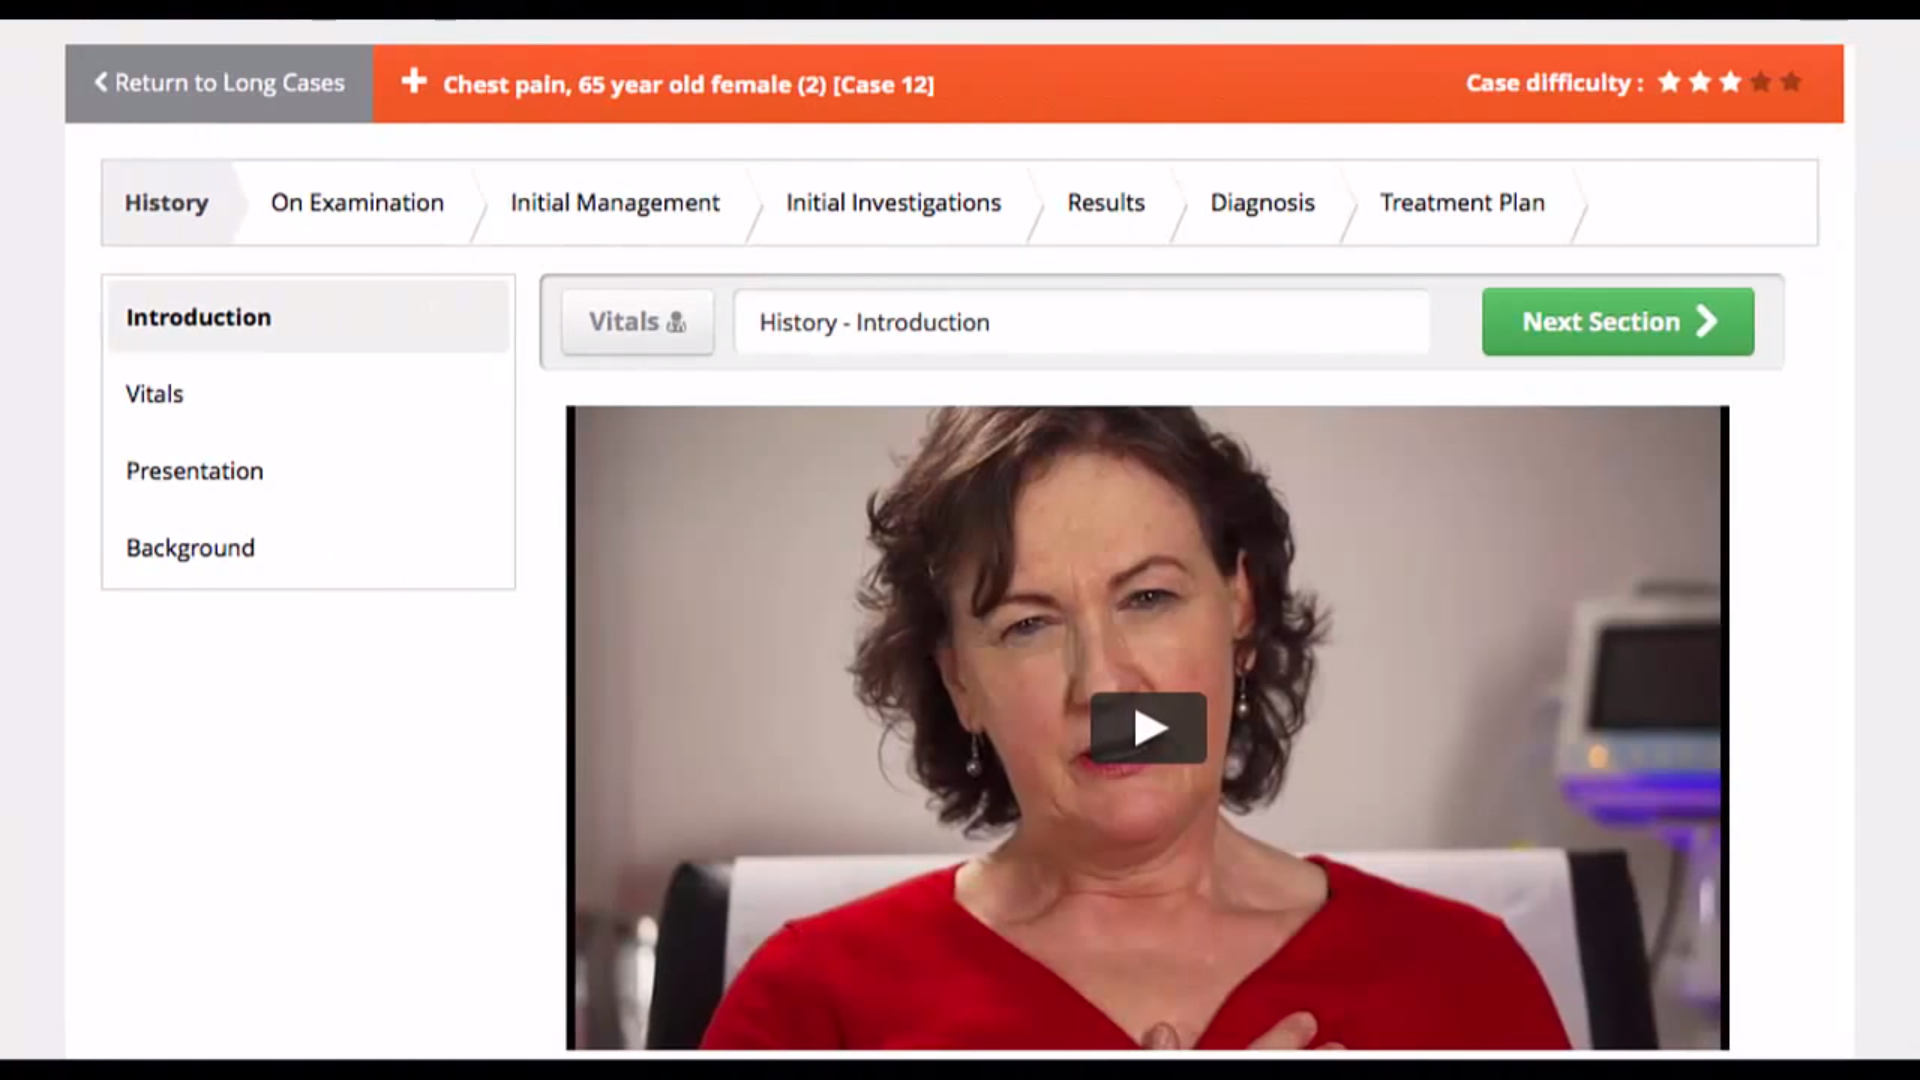
\includegraphics[width=0.9\textwidth]{figures/met/case choice.png}
    \captionsetup{justification=centering}
    \caption{Choix d'un cas}
\end{figure}

\subsubsection{Consultation des informations d'un patient}
L'apprenant a accès aux informations d'un patient. Les figures suivantes nous montre comment il a accès aux antécédents médicaux, aux allergies, aux paramètres et même à des scanner.
\begin{figure}
    \centering
    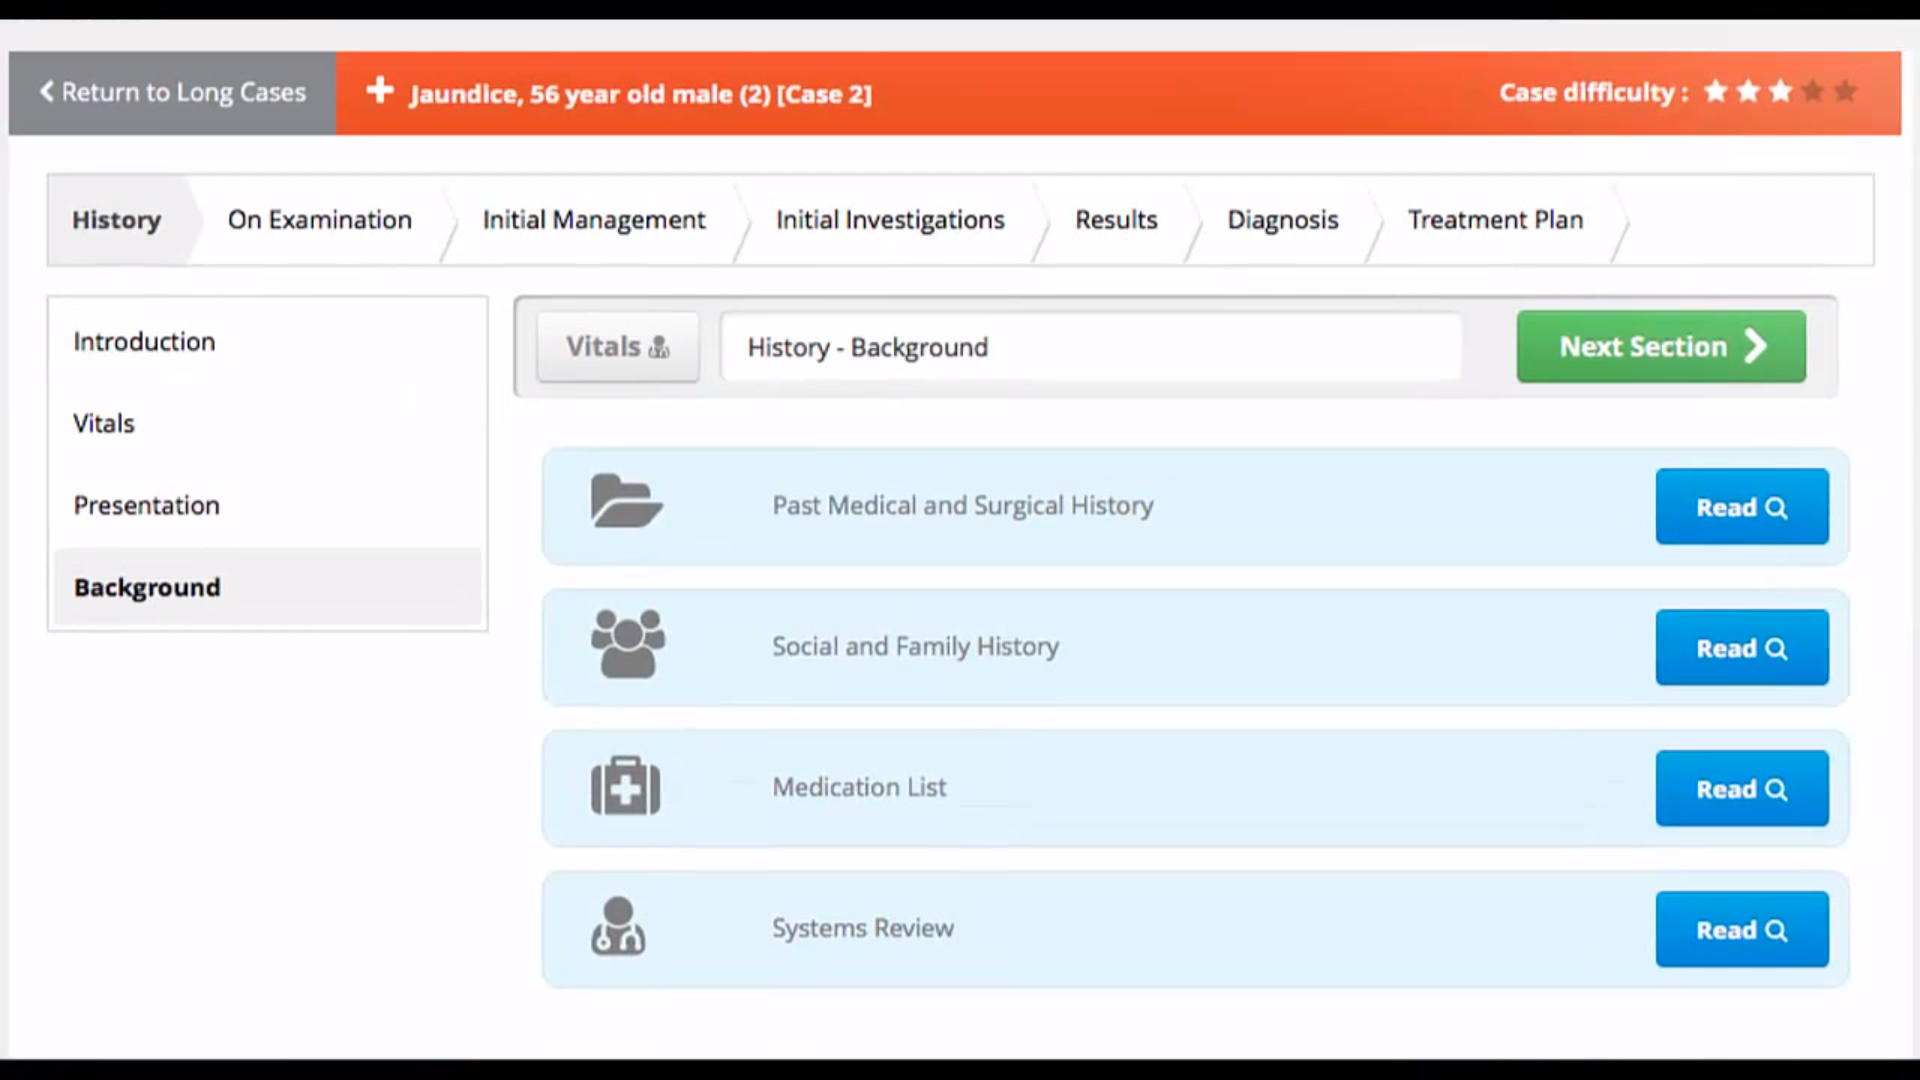
\includegraphics[width=0.9\textwidth]{figures/met/infos patient.png}
    \captionsetup{justification=centering}
    \caption{Informations d'un patient}
\end{figure}

\begin{figure}
    \centering
    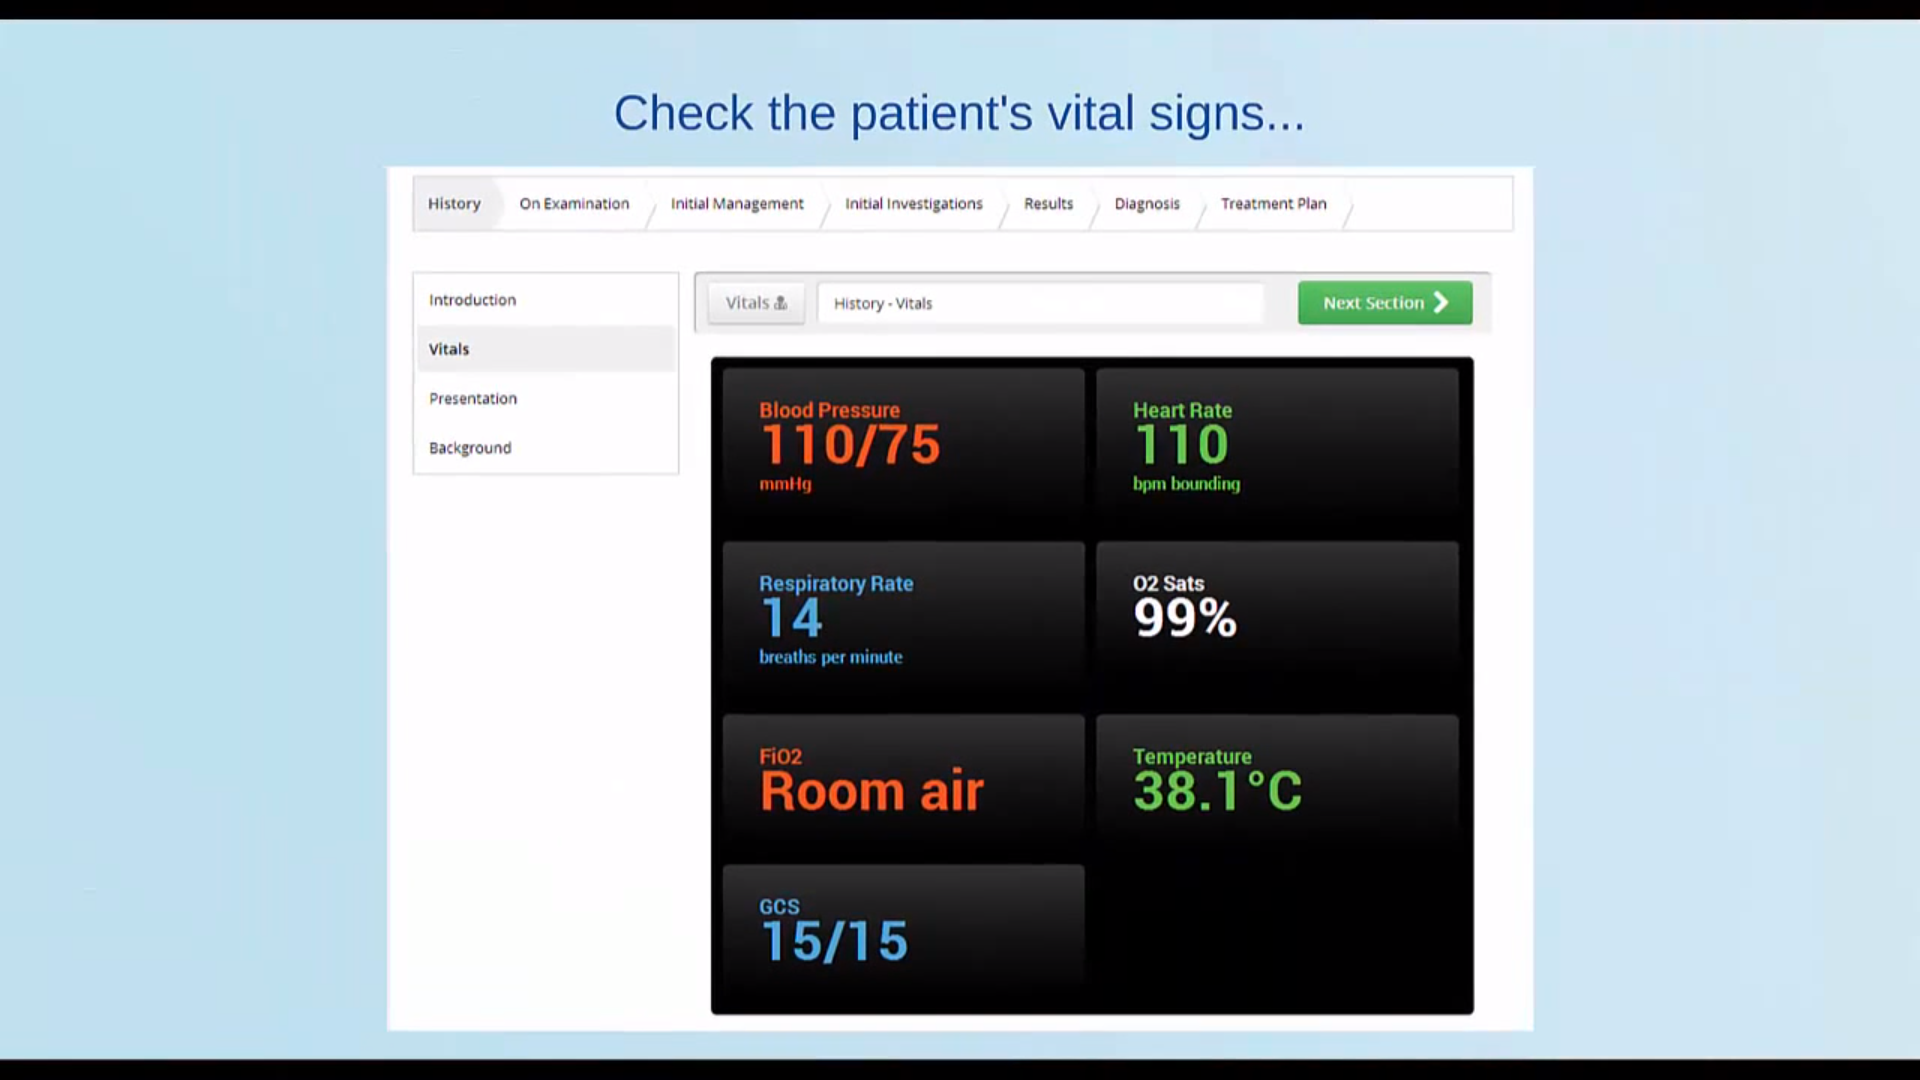
\includegraphics[width=0.9\textwidth]{figures/met/params.png}
    \captionsetup{justification=centering}
    \caption{Paramètres d'un patient}
\end{figure}

\begin{figure}
    \centering
    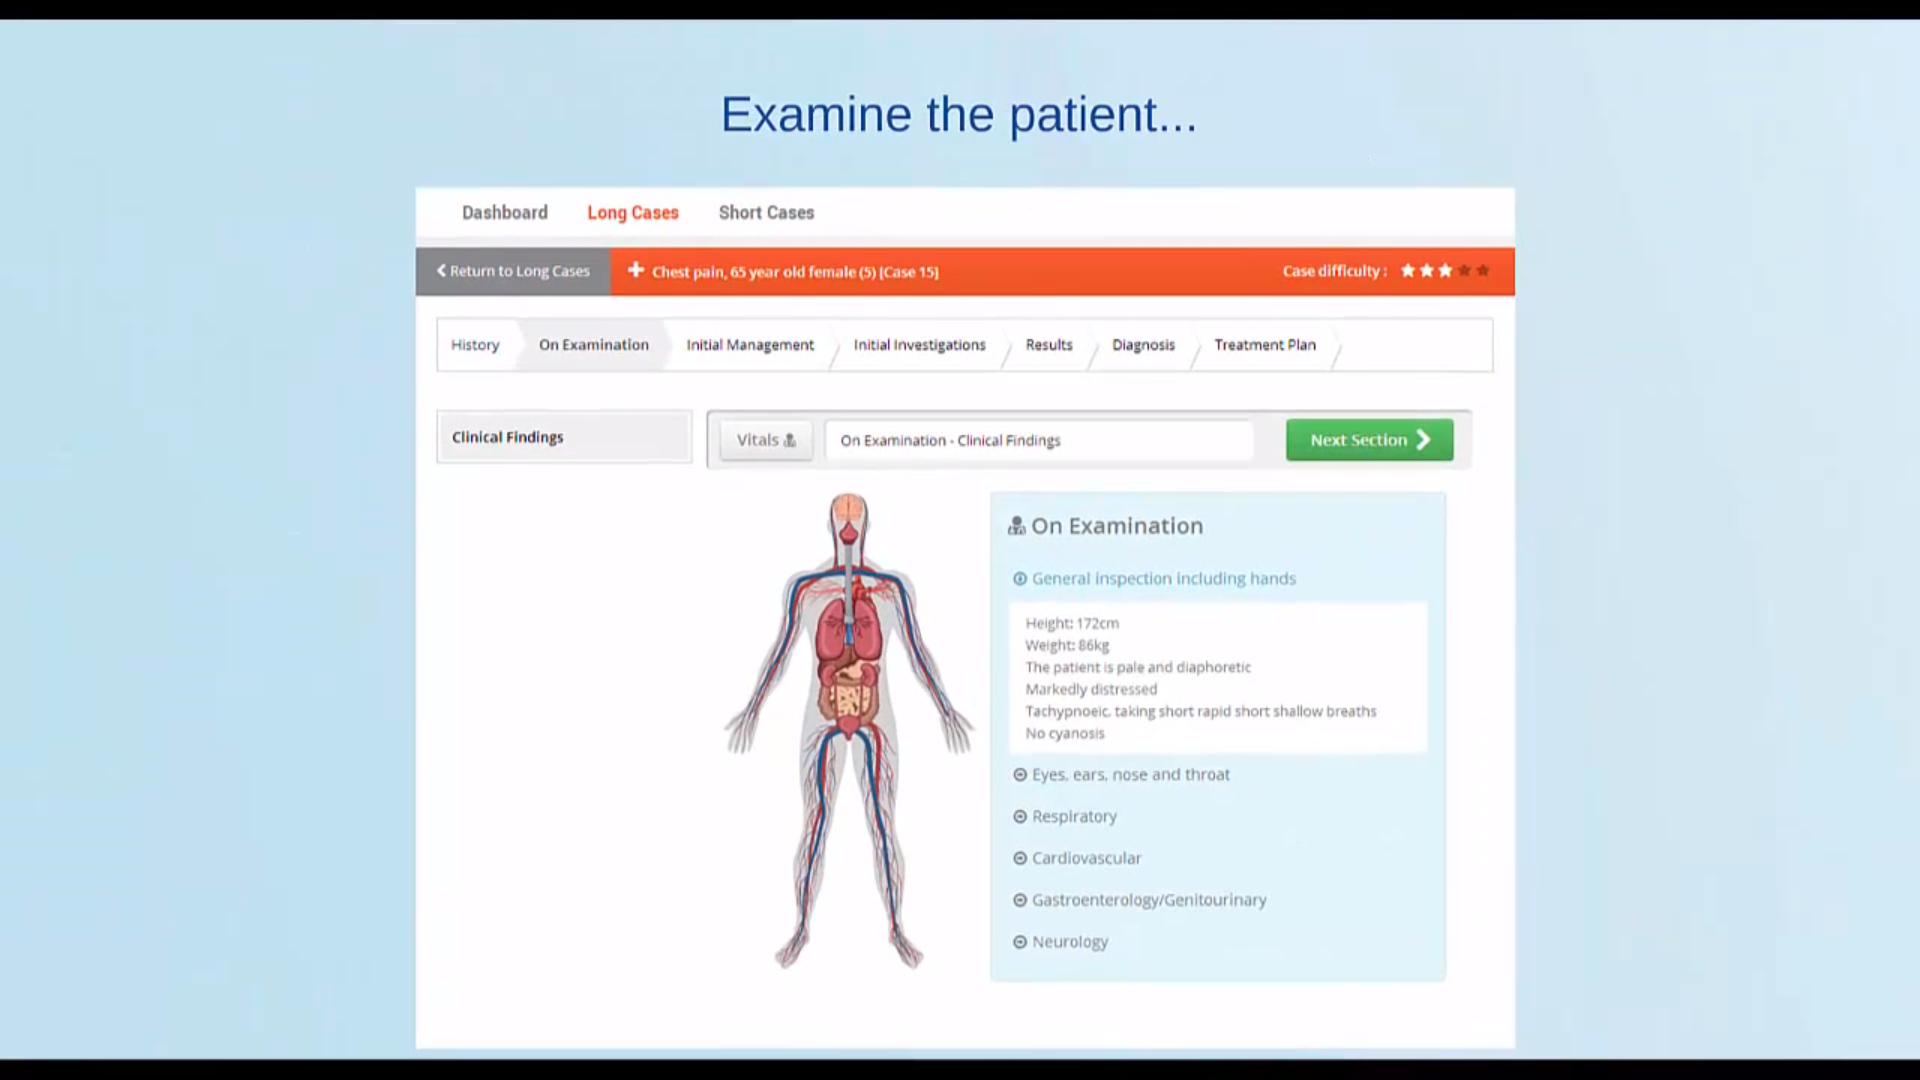
\includegraphics[width=0.9\textwidth]{figures/met/exam.png}
    \captionsetup{justification=centering}
    \caption{Examen d'un patient}
\end{figure}

\subsubsection{Limites}
Les limites de cette application sont directement liées aux challenge de l'enseignement du diagnostic médical. Le principal problème est le manque d'interaction entre le médecin apprenant et le patient, ce qui fait qu'un apprenant n'a pas le moyen d'apprendre comment faire un diagnostic, quelle question poser à un patient pour recueillir déjà dans la phase de l'interview des informations essentielles pour poser un diagnostique probable.

\subsection{Notre apport}
Dans ce travail, nous mettons l'accent non seulement sur l'enseignement de la capacité à établir des diagnostics fiables, mais aussi sur l'enseignement des bonnes pratiques à suivre par l'apprenant lors de la phase d'anamnèse.

Notre système s'appuie sur des cas réels choisis par des médecins experts pour établir les connaissances dans le domaine de la procédure d'anamnèse et pour la reconnaissance des maladies à partir des symptômes connus. De plus, nous fournissons des moyens pour évaluer grâce à un simulateur de patient virtuel comment un médecin apprenant s'y prends pour récolter des informations à partir d'un interview.


%reférence croisé \ref{chp:intro}


%Example of \autoref{alg:1} reference.
%\begin{algorithm}
%    \caption{Pseudocode}
%    \label{alg:1}
%    \begin{algorithmic}
%        \STATE $i\gets 10$
%        \IF {$i\geq 5$} 
%          \STATE $i\gets i-1$
%        \ELSE
%          \IF {$i\leq 3$}
%            \STATE $i\gets i+2$
%          \ENDIF
%        \ENDIF 
%    \end{algorithmic}
%\end{algorithm}